\begin{figure}
\begin{tabular}{@{}c@{}c@{}}
\begin{subfigure}[b]{0.5\textwidth}
\begin{center}
{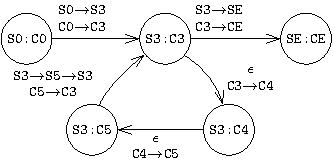
\includegraphics[scale=1.25]{chapters/figures/figMallocProductCfg.pdf}}
\end{center}
\caption{\label{figr:llAllocProductCFG}Product-CFG between CFGs \\ in \cref{fig:llAllocSpecIRCFG,fig:llAllocCCFG}}
\end{subfigure}%
&
\begin{subfigure}[b]{0.5\textwidth}
\begin{center}
\begin{footnotesize}
% \begin{table}
\begin{tabular}{cll}
\toprule
{\bf PC-Pair} & \multicolumn{2}{c}{\bf Invariants} \\
\toprule
(\scpc{0}{0}) & \multicolumn{2}{l}{ $\circled{P}\  \sv{n} = \cv{n}$} \\
\midrule
\multirow{2}{*}{(\scpc{3}{3})} &  $\circled{\scriptsize I1}\  \sv{n} = \cv{n}$ & $\circled{\scriptsize I2}\  \sv{i} = \cv{i}$ \\
&  $\circled{\scriptsize I3}\  \sv{i} \leq_{u} \sv{n}$ & $\circled{\scriptsize I4}\  \sv{l} \indEq{} \lifted{list}{\mem{}}{lnode}{\cv{l}}$ \\
\midrule
(\scpc{3}{4}) &  $\circled{\scriptsize I5}\  \sv{n}=\cv{n}$ & $\circled{\scriptsize I6}\  \sv{i}=\cv{i}$ \\
(\scpc{3}{5}) &  $\circled{\scriptsize I7}\  \sv{i} <_{u} \sv{n}$ & $\circled{\scriptsize I8}\  \sv{l} \indEq{} \lifted{list}{\mem{}}{lnode}{\cv{l}}$ \\
\midrule
(\scpc{E}{E}) & \multicolumn{2}{l}{ $\circled{E}\  \sv{ret} \indEq{} \lifted{list}{\mem{}}{lnode}{\cv{ret}}$} \\
\bottomrule
\end{tabular}
% \end{table}
\end{footnotesize}
\end{center}
\caption{\label{tabr:llproductInv}Node invariants for product-CFG in \cref{fig:llAllocProductCFG}}
\end{subfigure}%
\\
\end{tabular}
\caption{\label{figr:llallocProductCFGAndInvs}Product-CFG between the CFGs in \cref{fig:llAllocSpecIRCFG,fig:llAllocCCFG}.
\Cref{tab:llproductInv} contains the corresponding node invariants for the product-CFG.}
\end{figure}